\documentclass[12pt,letterpaper,twoside]{article}

\newif\ifsolution\solutiontrue   % Include the solutions
%\newif\ifsolution\solutionfalse  % Exclude the solutions

\usepackage{stats370}
\usepackage{xcolor}
\usepackage{float}
\usepackage{dsfont}
\usepackage{enumitem}
\usepackage{mathtools}
% \usepackage{breqn}
\usepackage{graphicx}
\usepackage[section]{placeins}
% \graphicspath{{output/}{\main/output/}}

\allowdisplaybreaks
\raggedbottom

\newcommand{\T}[1]{\text{\texttt{#1}}}
\newcommand{\V}[1]{\text{\textit{#1}}}

\begin{document}

{\centering \Large \textbf{Project: Sampling Methodologies \\}}
\vspace*{-8pt}\noindent\rule{\linewidth}{1pt}

\paragraph{Purpose} of the project is to compare different sampling methodologies 
for estimating the posterior $p(\theta|y_1,...,y_n)$ of a bayesian 
inference problem.

\paragraph{Data} $(y_1,...,y_n)$ are gene expression measurements for two genes 
on $n=24$ samples where $y_i=(y_{i,1}, y_{i,2})$ represent gene expressions for 
sample i. Our samples are all labelled by "group", denoted $(t_1,...,t_n)$. 
Cell type (or mix of cell types) vary with group and we assume mean gene 
expression (but not variance) depends on cell type. Moreover, the expressions 
of different genes are independently normally distributed.

\begin{itemize}
    \item $Y_i \sim N(\mu, \sigma^2 \mathbb{I})$ if sample $i$ from group 1
    \item $Y_i \sim N(\gamma, \sigma^2 \mathbb{I})$ if sample $i$ from group 2
    \item $Y_i \sim N(0.5\mu + 0.5\gamma, \sigma^2 \mathbb{I})$ if sample $i$ from group 3
    \item $Y_i \sim N(\tau\mu + (1-\tau)\gamma, \sigma^2 \mathbb{I})$ if sample $i$ from group 4
\end{itemize}

Our model has a 6-dimensional parameter $\theta = (\sigma^2, \tau, \mu_1, \mu_2, \gamma_1, \gamma_2)$.

For all sampling methodologies, I computed 5000 samples with a 
burn-in of 200. The rest (step size, momentum, proposals, etc.) I 
discuss and treat as design choices.


% \newpage
\section{Metropolis Hastings}
To implement the Metropolis-Hastings algorithm we require the 
joint and transition densities to compute the hastings ratio. 
Below we derive the join density for our model, and treat the 
transition density as a design choice.

\textbf{Joint density}:
\begin{align*}
    p(\theta|y) & \propto \prod_{i=1}^n p(y|\theta) p(\theta) \\
                & = \prod_{t=1}^4 \prod_{i=1}^n 1\{t_i=t\} \cdot p(y_i|\theta) \cdot p(\mu) \cdot p(\gamma) \cdot p(\tau) \cdot p(\sigma^2) \\
                & = \prod_{t_i=1} N(\mu, \sigma^2 \mathbb{I}) \cdot \prod_{t_i=2} N(\gamma, \sigma^2 \mathbb{I}) \cdot \prod_{t_i=3} N(0.5\mu + 0.5\gamma, \sigma^2 \mathbb{I}) \cdot \prod_{t_i=4} N(\tau\mu + (1-\tau)\gamma, \sigma^2 \mathbb{I}) \cdot p(\sigma^2)
\end{align*}

\textbf{Hastings Ratio}: let $q(\theta_0, \theta_1)$ be our transition density and 
$\pi(y,\theta)$ be our join density. Then, 
$$\text{accept prob.} = \min(1, \frac{q(\theta_0, \theta_1)\pi(y,\theta_1)}{q(\theta_1, \theta_0)\pi(y,\theta_0)})$$

\begin{python}
def metropolis_hastings(data, n_samples, step_size, inital_position):
    curr_theta = inital_position.copy()
    samples = [curr_theta]

    while it < n_samples:

        proposed = proposal_sampler(curr_theta, step_size)
        h_ratio = hastings_ratio(proposed, curr_theta, data)
        accept_prob = min(1, h_ratio)

        if np.random.uniform(0, 1) <= accept_prob:
            curr_theta = proposed
            accept_count += 1

        samples.append(curr_theta)

    return samples
\end{python}

The Metropolis-Hastings algorithm itself is very simple,
However, there are still a number of design choices we need to make, 
such as (a) how to propose a new sample, (b) enforcing any constraints 
we have (e.g. $\tau \in [0,1]$), and (c) choosing hyperparameters (step 
size, burn-in).

\begin{enumerate}[label=(\alph*)]
\item \textbf{Enforcing constraints}: We had two constraints to consider: (a) $\sigma^2 > 0$ 
and (b) $0 \le \tau \le 1$. I enforce these constraints for our symmetric proposal method by resampling 
if the proposal violates either (a) or (b). This reduces the efficiency (acceptance ratio) of 
the algorithm substantially and introduces potential bias in our resulting marginal posterior 
samples (particularly for $\tau$ which has significant density near its upper bound, mean shifted 
from ~0.75 to ~0.85). By contrast, our asymmetric proposal method encodes these constraints directly. 
For these reasons, we use the asymmetric kernel for our results.

\item \textbf{Hyperparameters}: There are not many hyperparameters to 
tune for Metropolis-Hastings, which is one of its advantages! I 
experimented with different step sizes (0.01, 0.05, 0.1, 0.5), 
and for each computed the acceptance ratio and mean number of 
effective (uncorrelated) samples for 300 sample test (after 
burn-in). I choose a step size of 0.05 since it maximized 
both number of effective samples and acceptance ratio.

\begin{table}[H]
    \centering
    \begin{tabular}{lllll}
        Step size                   & 0.01 & 0.05  & 0.1   & 0.5   \\
        Acceptance ratio            & 0.87 & 0.44  & 0.22  & 0.02  \\
        Effective samples           & 3.5  & 16.6  & 14.6  & 6.96  \\
                                    &      &       &       &         
    \end{tabular}
\end{table}

I did not investigate varying initialization (used $[1., 0.5, 0., 0., 0., 0.]$)
or burn-in (fixed at 200 to match what I saw in textbook examples).
\end{enumerate}

\textbf{Results}: Using the above design choices, we produce the following 
samples from our posterior (Figure 1) and compute the first and second 
moments (table below). These passed basic sense checks, such as $\sigma^2$ 
and $\tau$ falling within their respective bounds, mean and variance matching 
results from other sampling algorithms, and lower variance as we increase number 
of samples.
\begin{figure}[H]
    \centering
    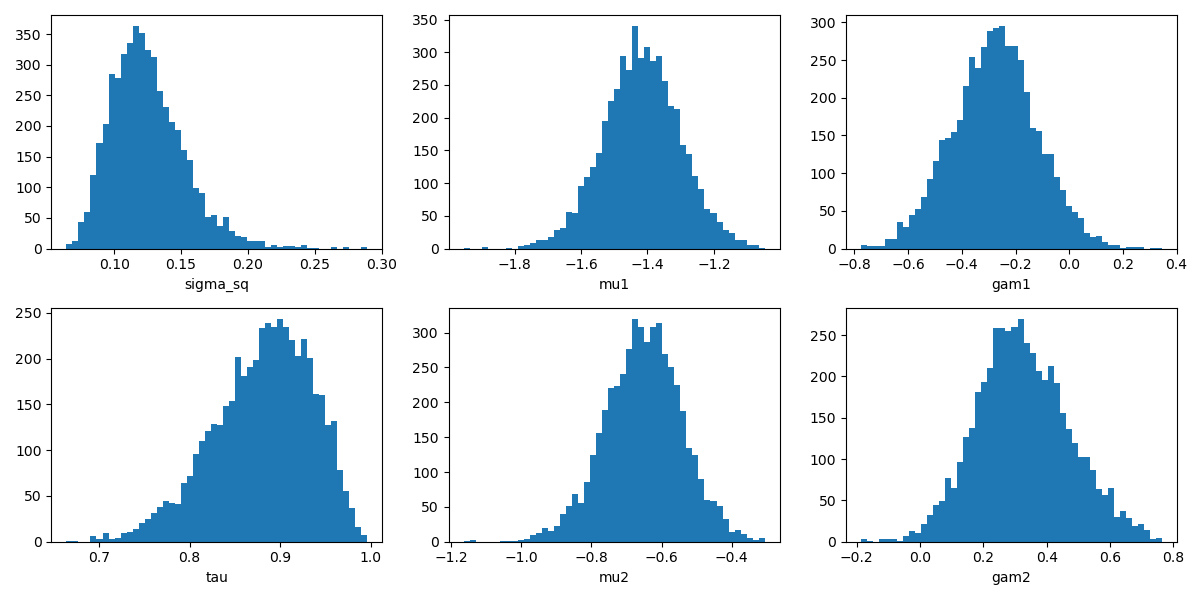
\includegraphics[scale=0.55]{images/histogram.png}
    \vspace*{-10mm}
    \caption{Histogram of Metropolis-Hastings posterior samples}
\end{figure}

\begin{table}[H]
    \begin{tabular}{lcccccc}
    \multicolumn{1}{c}{}          & sigma$^2$ & tau   & mu1   & mu2   & gam1  & gam2  \\
    Mean of posterior samples     & 0.14  & 0.84  & -1.44 & -0.67 & -0.25 & 0.35  \\
    Variance of posterior samples & 0.004 & 0.008 & 0.015 & 0.023 & 0.022 & 0.025
    \end{tabular}
\end{table}

\textbf{Final remarks}. Metropolis-Hastings is simple to implement 
and relatively fast to run (time = 197 sec for 5000 samples), however,
number of effective samples (autocorrelation) and acceptance ratio 
were not as good as we might expect from other technqiues that take 
more directed paths through the posterior space (e.g. HMC).   

\end{document}
